\documentclass{article}
\usepackage{hyperref}
\usepackage{graphicx}
\graphicspath{ {images/} }

\title{User Manual}
\author{devs101}

\begin{document}
\maketitle
\tableofcontents
\newpage

\section{Introduction}
This user manual will guide the user through getting the Trii up and running and show them how to add nodes to the graph.
\section{General Information}
\subsection{Title Page}
Trii by Devs101
\subsection{System Overview}
A skill tree is a graphical representation of the players current skills they have unlocked, the skills they can unlock and the dependencies the skills have on one another. This allows user to create custom configuration of the character's skills. Trii allows users the ability to design complex and powerful skill trees with little to no effort. The skill tree that is designed can then be exported as a .js file or a json file to be used later on. If the user so wishes they can import a tree from a json file.
\subsection{System Configuration}
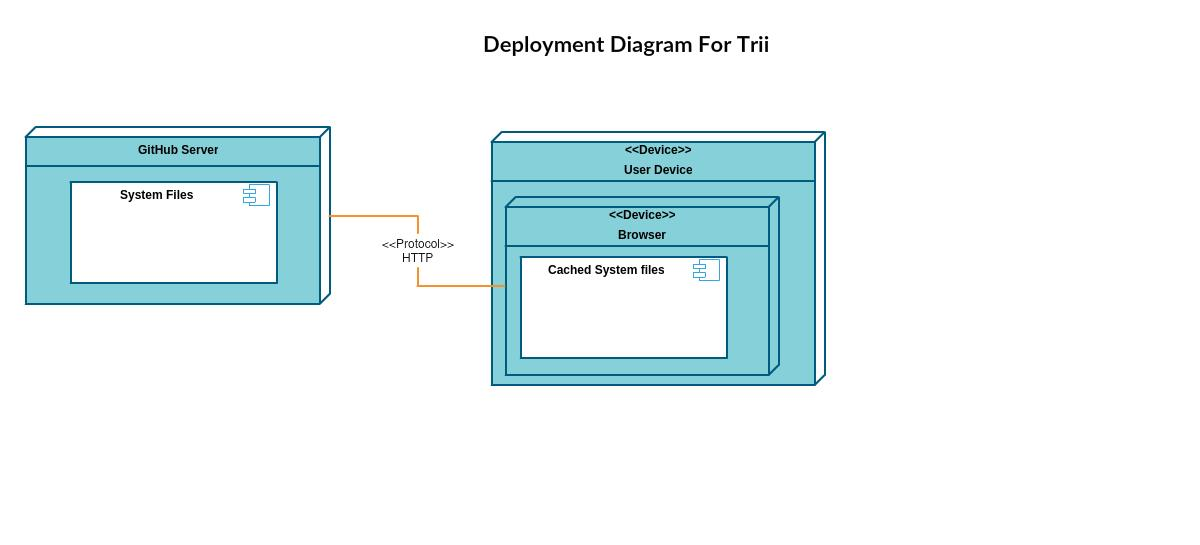
\includegraphics[scale=0.3]{deployment}\\
\subsection{Installation}
The software can be accessed at https://dolan212.github.io.
\section{Getting started}
In order to access Trii an internet browser with an active internet connection is required for the first access. After the first time it has been accessed it can be accessed through the browser at anytime whether there is an active internet connection or not. In terms of accessing Trii the reccommended internet browser is Google chrome which can be downloaded here: https://www.google.com/chrome/ or on your mobile devices respective application market place. The system can now be accessed at https://dolan212.github.io .
\section{Using the System}
Once the system has been launched the user will be shown this page:\\
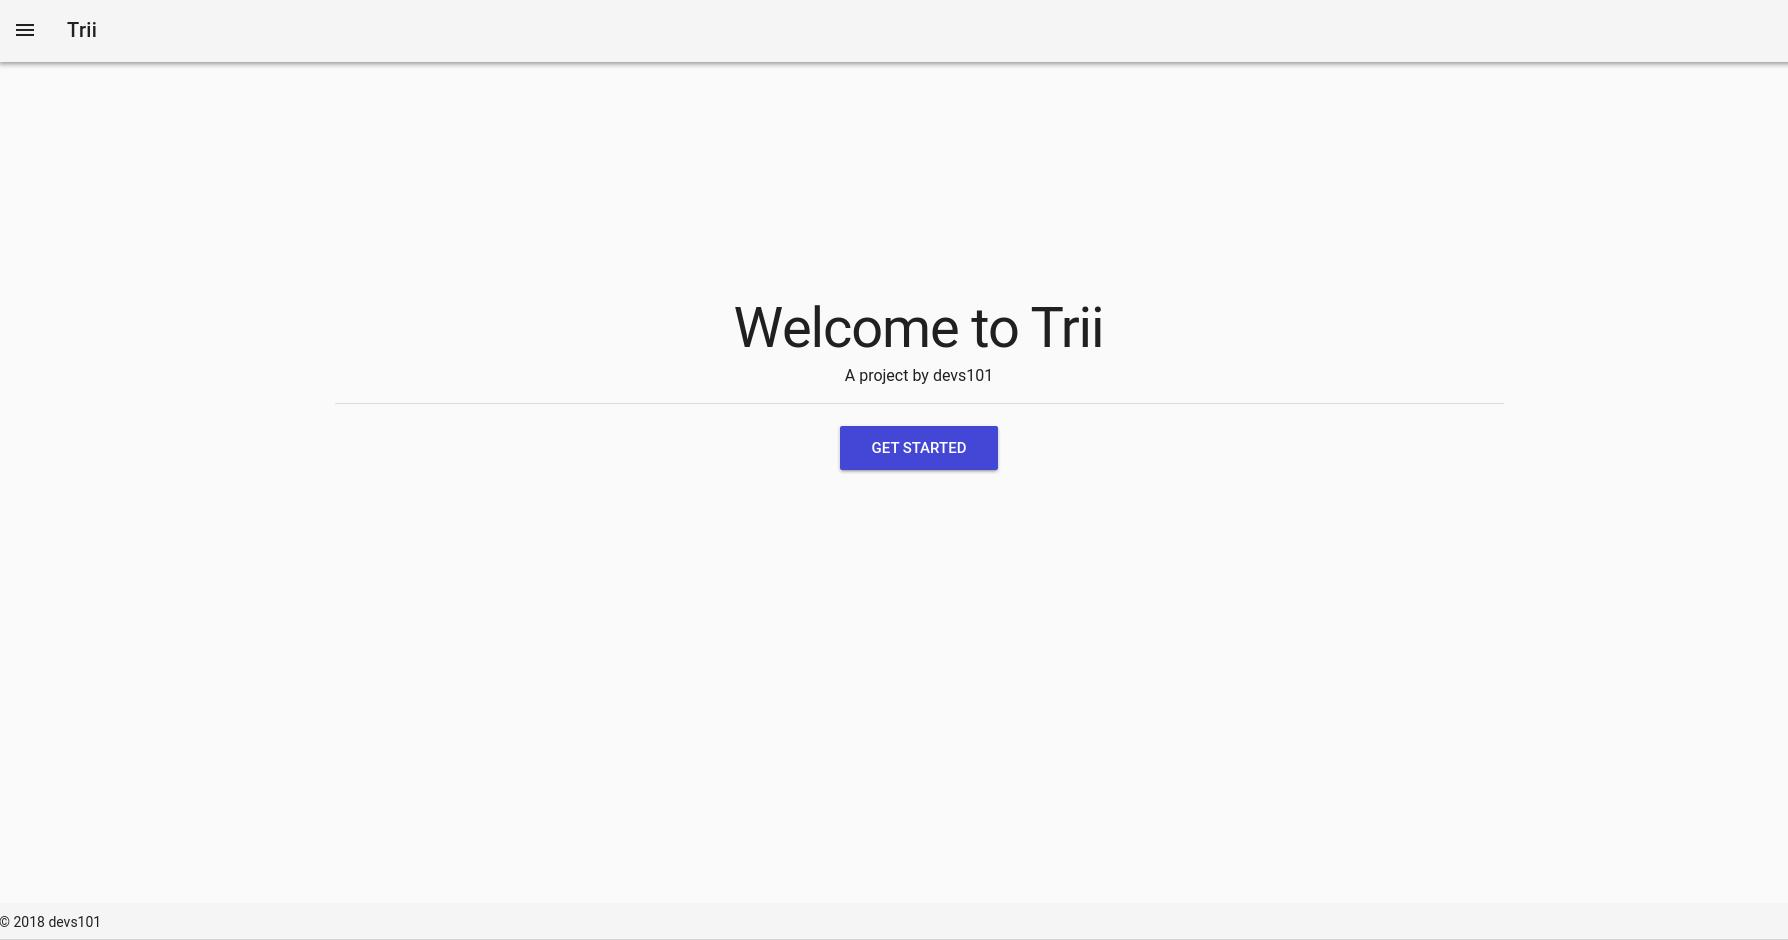
\includegraphics[scale=0.25]{landingpage}\\
To get started the user will need to click the get started button. Once the button has been clicked the user will be show a page which looks like this:\\
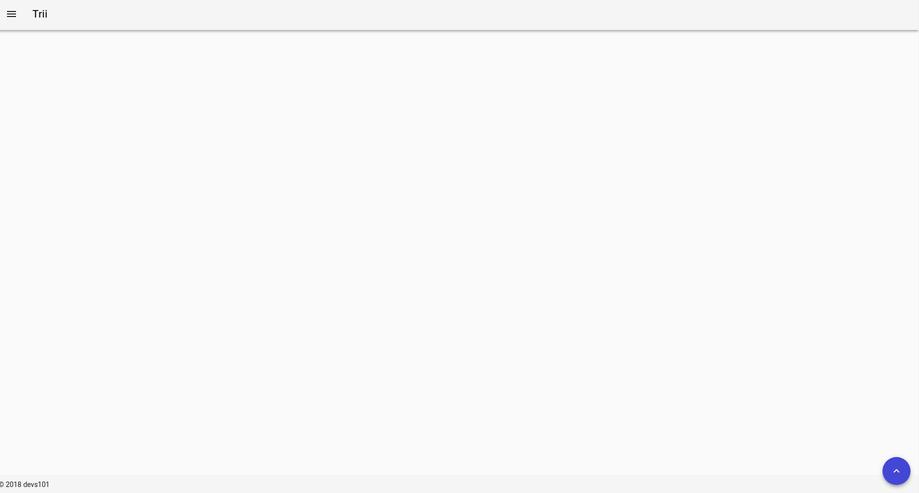
\includegraphics[scale=0.49]{treeView}\\
from this view the user will be able to add nodes.\\
This can be done by clicking the circular button in the bottom right corner of the screen which will produce the following view.\\
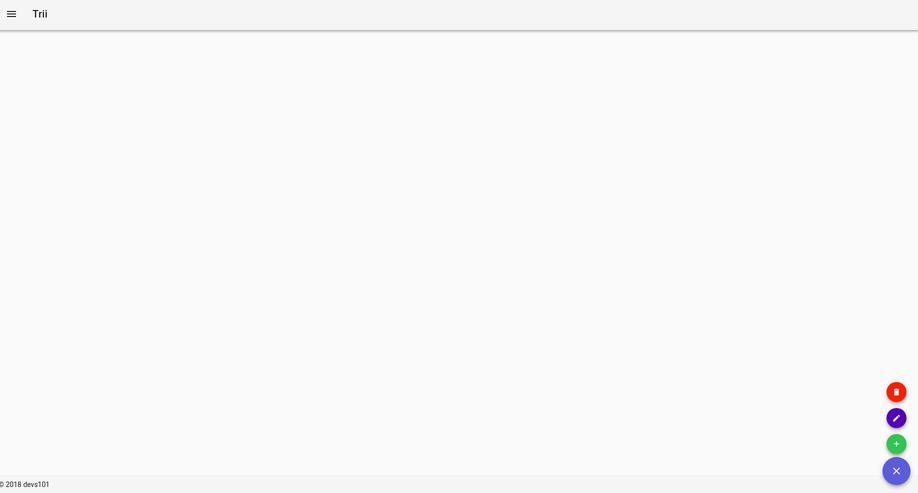
\includegraphics[scale=0.49]{fabSelected}\\
The user can then click the green circular button with the plus sign on to add the node. Once clicked a dialog will popup asking the user to add in give the node a label. Once the node has been given a label the user can click on add in the dialog and the node will be added.
\section{Troubleshooting}
If while trying to add a new node the labels text box is populated with a previous nodes name just clear the text box.

\end{document}
